\documentclass[10pt,a4paper]{article}

\newcommand{\reportauthors}{GIAP Tran Hoang}
\newcommand{\reportrepo}{\url{https://github.com/hoanggiaptran130503-bot/cv7001_ml_mini-project.git}}
\newcommand{\validationmae}{0.00917}
\newcommand{\validationmse}{1.82\times 10^{-4}}

\usepackage[margin=20mm]{geometry}
\usepackage[T1]{fontenc}
\usepackage{lmodern}
\usepackage{microtype}

\usepackage{graphicx}
\usepackage{float}
\usepackage{booktabs}
\usepackage{amsmath}
\usepackage[colorlinks=true,urlcolor=blue!55!black,linkcolor=blue!55!black]{hyperref}
\usepackage{xcolor}

\setlength{\parindent}{0pt}
\setlength{\parskip}{4pt}
\setlength{\textfloatsep}{9pt}
\setlength{\intextsep}{9pt}

\begin{document}
\begin{center}
{\Large\bfseries Predicting Reinforced-Concrete Wall Design Quantities with a DFNNs model\par}
\vspace{5pt}
{\normalsize \reportauthors\par}
\vspace{2pt}
{\small Course: Machine Learning Mini-Project \quad | \quad \reportrepo\par}
\end{center}
\vspace{-6pt}

\section{Problem and Motivation}
This project examines whether a deep feed-forward neural network (DFNN) can
approximate design decisions for a reinforced-concrete wall in one building.
The inputs are axial force $P$, bending moment $M_3$, and wall length $L_w$.
The outputs are edge-region length $B$, wall thickness $t$, and provided
reinforcement area $A_{s,\mathrm{prov}}$. The intended use is rapid estimation
for similar cases within the studied building; a prediction is not a completed
structural design check.

\section{Dataset and Method}
The project generated the input forces from their finite-element building
model and the target dimensions and reinforcement from their capstone design
workflow. The machine-learning dataset contains 155 paired samples with three
inputs and three targets. The first 139 samples (90\%) were used for training
and the final 16 (10\%) for validation. Five separately designed cases, absent
from the training dataset, were reserved for a final comparison. The scripts
read preprocessed numerical inputs and normalized targets; the normalization
procedure and the applied Eurocode edition must be specified in the repository.

The input data is processed through threes hidden layers with 72 nodes each. Each node combines inputs from the previous layer with unique weights and a bias term, adding flexibility to the model. This combined input is then transformed using an exponential linear unit (ELU) activation function, which introduces nonlinearity, allowing the network to learn intricate patterns and address the vanishing gradient issue for smoother training (Figure~\ref{fig:dfnn}).

\begin{figure}[H]
\centering
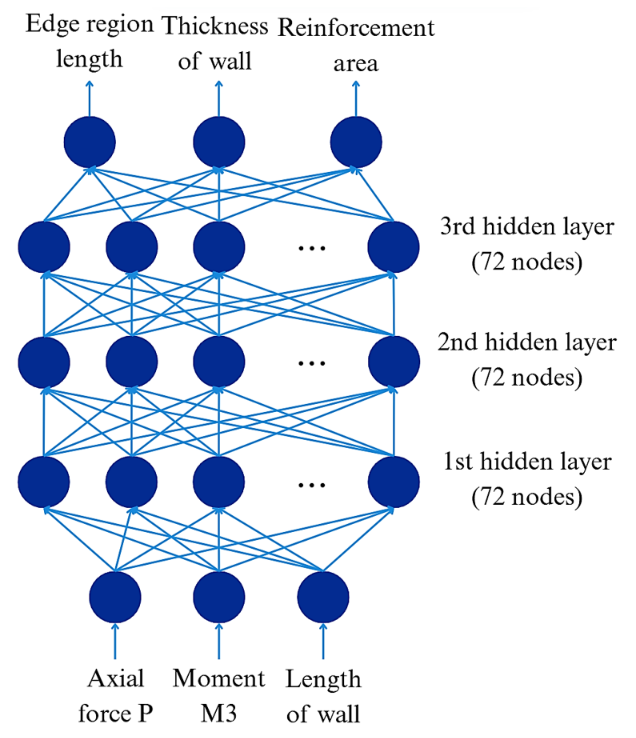
\includegraphics[width=0.40\linewidth]{Picture1.png}
\caption{DFNN architecture.}
\label{fig:dfnn}
\end{figure}

It was trained with mean-squared-error loss,
Adamax optimization, and early stopping using validation loss. The training
script permits up to 1500 epochs with batch size one. On the 16 validation
samples, the saved model achieved $\mathrm{MAE}=\validationmae$ and
$\mathrm{MSE}=\validationmse$ on the normalized target scale.

\section{Results and Discussion}
The validation curves show a persistent gap between training and validation
errors: the lowest validation loss occurred after the first epoch, although
training loss continued to decrease. The five separate design cases were then
compared with the DFNN predictions. For each output, the signed relative
difference is $d=100(y_{\mathrm{design}}-\hat y_{\mathrm{DFNN}})
/y_{\mathrm{design}}$. Table~\ref{tab:test} reports $|d|$, matching the
absolute-value formula in the saved comparison workbook. These percentages
were calculated from the paired normalized values in that workbook.

\begin{table}[h]
\centering
\caption{Absolute relative difference between design and DFNN prediction (\%).}
\label{tab:test}
\begin{tabular}{lccc}
\toprule
Case & $B$ & $t$ & $A_{s,\mathrm{prov}}$ \\
\midrule
1 & 0.9 & 1.6 & 3.0 \\
2 & 5.6 & 2.0 & 7.6 \\
3 & 4.6 & 0.2 & 1.5 \\
4 & 13.3 & 5.3 & 0.2 \\
5 & 2.1 & 7.7 & 2.4 \\
\midrule
Mean & 5.3 & 3.4 & 2.9 \\
\bottomrule
\end{tabular}
\end{table}

According to Table~\ref{tab:test}, most of differences are less than 5\%. The five cases provide a within-building comparison against existing design
values. They do not establish performance for other buildings, structural
systems, or load ranges. The validation gap and limited set of distinct target
combinations warrant caution when interpreting the small case-wise percentage
differences.

\section{Conclusions and Reflection}
The DFNN approximated the design targets of the five selected cases with the
relative differences shown in Table~\ref{tab:test}; validation performance
was weaker than training performance. Because its training targets
were produced by a Eurocode-based design workflow, its outputs may reflect
patterns in that workflow; agreement with the targets does not demonstrate
Eurocode compliance. Future work should convert predictions to practical
detailing choices and verify the resulting wall design against the applicable
resistance and detailing requirements.

\section*{Reproducibility and Disclosures}
The repository should provide the dataset, the saved model, installation
requirements, and exact commands to retrain and evaluate Cases 1--5.

The dataset and initial model code were adapted from the authors' capstone
project.

\begin{thebibliography}{9}
\setlength{\itemsep}{0pt}
\bibitem{tensorflow} TensorFlow Developers. \emph{TensorFlow} (software).
\url{https://www.tensorflow.org/}.

\bibitem{eurocode} CEN. \emph{BS EN 1992-1-1:2023 -- Eurocode 2: Design of concrete structures}.
TODO: applicable National Annex.
\end{thebibliography}
\end{document}
